\chapter{Point Cloud Registration} \label{ch:pcreg}
The main subject of this paper is two register two or more point clouds. The goal of registration is to find the rigid transformation(s) that will put the point clouds in one common coordinate system. Applying this transformation will make the point clouds overlap, making surfaces of the object that occur in both overlap. The term ``alignment'' is used interchangeably with ``registration'', though the former emphasizes that \emph{surfaces} are being aligned.

For registration to be meaningful, the hypothesis is made that the point clouds do represent scans of the same object, and that the \emph{true} rigid transformation(s) that align them exist. For the case of two 3D scans of a stationary object, this true transformation would be the pose of the first scan relative to that of the second scan. The goal of registration algorithms is then to find an estimation of the true transformation. Except for artificially generated testing data, the true transformation is usually unknown or known only at a limited precision.

This chapter consists of a classification and survey of existing registration methods.

\section{Introduction}

\emph{Pair-wise} registration algorithms take one \emph{fixed} point cloud $P$ and one \emph{loose} point cloud $Q$ as input. The output is a rigid transformation $\emph{M}$ that brings $Q$ into the coordinate system of $P$. During the algorithm $P$ is left unchanged, while $Q$ is being moved around. Thus implementations can preprocess $P$ once to allow for more efficient computation, for example by representing it in a KdTree, so that closest points can be computed more quickly. The representation of $Q$ on the other hand may be modified on the fly, for example by applying a partial transformation to the points' coordinates at each iteration of the algorithm.

When the goal is to register multiple point clouds $\{ P_i \}$, a pair-wise algorithm would be applied multiple times to different pairs $(P_i, P_j)$. Depending on how these pairs are chosen, this leads to an accumulation of the registration error. \emph{Multi-view} registration algorithms instead directly operate on a set of point clouds to align, and aim to evenly distribute the registration error. The output is a set of rigid transformations $\{ \matr{M_i} \}$, one for each input point cloud. (If one point cloud $P_f$ is chosen as fixed, then $\matr{M_f} = \matr{I}$)

A primary distinction is made depending on whether an initial estimation for $\matr{M}$ is already known. This may come for example from manual alignment made in a 3D visualizer application, or from sensors attached to the scanners that detect its pose. \emph{Coarse registration} algorithms make no such assumption and use a representation of the point cloud that is invariant to its current pose relative to the other one, to deduce an approximate alignment. \emph{Fine registration} algorithms assume that the point clouds are already approximatively registered, and improve upon the alignment by bringing corresponding parts closer together. The goal is to obtain the most accurate solution possible. Some methods can also yield a fine registration, without initial registration.

In the most usual case the point clouds to register already have the same scale, so $\matr{M}$ is a proper rigid transformation. When this is not the case, for example when one of the point clouds was taken using photogrammetry and the real scale is unknown, the goal would additionally be to find a scaling factor. $\matr{M}$ would then be a composition of a proper rigid transformation followed by a scaling transformation.

There is also the notion of \emph{non-rigid registration}, which is a generalization where the loose point clouds can also be deformed. The output is no longer a single (rigid or otherwise) transformation matrix. Depending on the deformation model used, it may instead be a per-point displacement field, or a rigid transformation combined with a modification of a skeleton that parametrizes the deformation. It is used to to register point clouds depicting one same object that can change shape in some limited way between the scans, for instance a waving flag, a human face or in medical imaging an internal organ. This this paper only rigid registration is considered.


\section{Robustness} \label{sec:registration_robostness}
The ideal case for registration of two point clouds $P$ and $Q$ would be if $P = \{ \matr{M} \, p : p \in P \}$, that is they both contain exactly the same constellation of points, with $Q$ being transformed by precisely the \emph{true} rigid transformation $\matr{M}$. Here one unique (unless the model has precise rotation symmetry) rigid transformation $\matr{M}$ exists which makes $P$ and $Q$ coincide, and it is possible for a trivial algorithm to compute $\matr{M}$ at an arbitrary level of precision, taking only $P$ and $Q$ as input.

However in practice $P$ and $Q$ will differ in many more ways than the rigid transformation. A registration algorithm is deemed \emph{robust} if it continues to deliver good results when the disparities between the point clouds get progressively worse.

The disparities can for example be the following:
\begin{description}
\item[Points dispersion] The points of a point cloud constitute a discrete subset of the surfaces that are represented. Unless $P$ and $Q$ were algorithmically generated from one scanner output file, those subsets will be different but still approximate the same surface. The lower the point density, the stronger this disparity becomes.

Points on a planar surfaces will typically be dispersed approximatively on a quadrilateral grid, when scanned using a laser scanner that proceeds in sequential scan-lines. It becomes a square grid on surfaces facing the scanner. The more the surface is oblique, the wider the rectangles get and the density gets lower.

When large objects are scanner, the points density will naturally get lower on surface locations further away from the scanner. 

\item[Noise] One or both point clouds can contain outlier points that do not lie on any relevant surface of the model. They result from points that were scanner from the environment but are not part of the model surfaces, scanner errors, or artifacts from prior processing.

A good registration algorithm should be insensitive to outlier points, or be able to identify them and sort them out before continuing. The \emph{noise-to-signal} ratio can be defined as the number of outlier points divided by the number of inlier points.

\item[Bounds] The two point clouds contain only points within given geometric bounds, either due to the limited range and field of view of the scanner, or from having been cropped out of a larger point cloud in preprocessing.

While a minimal bounding box, frustum, etc. can be computed from a point cloud such that all its points are within it, the actual bounding region is usually not known. That is, if there is no point in a particular location, it is not immediately known whether this is because there is no object surface at that location of because the location is out of bounds. (For range images, the field of view is known.)

But all points that are not within the intersection of those bounding regions of $P$ and $Q$ will have no corresponding point in the other point cloud, and so they need to be treated by the algorithm the same way as outliers.

\item[Occlusion] The scanner can only record surface points that are visible from its pose. So occluded areas will not be covered by the point cloud. Because no surface connectivity information is recorded, and sometimes the scanner position in the point cloud coordinate system is unknown, it becomes hard to tell what regions are occluded. Moreover because the surfaces are only partially covered, reconstructing them becomes a harder problem.

When registering two scans taken from different poses, their region of overlap becomes limited to the areas that are not occluded in either point cloud. Point outside it will have not corresponding point in the other cloud. But they still hold information about the underlying surface that is represented by both $P$ and $Q$.
\end{description} 


\section{Fine registration}
As stated, fine registration algorithms take as input two (or more) point clouds that are already approximatively aligned, and then improve their alignment as much as possible. The core observation is that corresponding points in the two point clouds are already close to each other in the current alignment.

\subsection{Iterative Closest Point} \label{sec:icp}
The most well-known fine registration algorithm is Iterative Closest Point (ICP), first described in \cite{Besl1992} and in \cite{Chen1991}. It is a pair-wise algorithm, though multi-view versions of it also are also possible \cite{Told2010}.

The algorithm chooses \emph{point correspondences} $(p \in P, q \in Q)$, where $q$ is the point closest to $p$ with the current alignment. Using the assumption that $P$ and $Q$ are already roughly aligned, those correspondences approximatively correspond to real corresponding point in both representations of the object. Then a rigid transformation is applied to $Q$ which minimizes the distances $d(p, q)$ for all corresponding point pairs in a least squares sense. The process is repeated iteratively.

Different terms for the fixed and loose point clouds are frequently used in the literature. For example the fixed point cloud may be called ``model'', ``target'' or ``reference'', the loose one may be called ``data'' or ``source''. In this text the terms ``fixed'' and ``loose'' are used.

\subsubsection{ICP framework}
There are many possible variations of ICP algorithms \cite{Rusi2001}. For all of them the following 6 steps are performed at each iteration:
\begin{description}
\item[Selection] Select a subset of points from $P$ and/or $Q$ to consider. In the simplest case all points are considered. Alternatives include the selection of a random subset with a given \emph{downsampling ratio}. The decision to include or reject a point, or the probability of including a given point, may depend on a given metric, such as its distance to the center, distance to the closest neighbour, orientation of normal vector, and others. Here the selected subsets are called $P^*$ and $Q^*$ respectively.
\item[Correspondence] Build correspondence pairs $(p_i, q_i)$ using the selected points. The \emph{closest point criterion} is to choose for each $p \in P^*$ the point $q \in Q^*$ (or the other way) whose Euclidian distance $\|p - q\|$ to it is minimal. Here $p_i$ and $q_j$ denote corresponding points when $i = j$. It is not necessarily a one-to-one mapping: A point from one cloud may correspond to multiple point from the other.

There are other strategies for choosing point correspondences. When the normal vectors $\vec{n_p}$ are known, one possibility is to choose $q \in Q^*$ that is closest to the ray pointing out of $p$ in the direction of its normal vector $\vec{n_p}$. Also it can be useful to only consider points in $Q^*$ that satisfy certain constraints in function of $p$, such as a similar normal vector orientation, color, or other.

It is also not necessary for both $P$ and $Q$ to be point clouds. For example $Q$ may instead be defined using a parametric surface. For each $q$ a corresponding point $q$ is then computed from $p$, instead of chosen from a finite set.

Finding correspondences is typically the most computationally intensive operation in the ICP iterations. One way to optimize closest point finding it is to use an appropriate data structure for $Q$, for example a KdTree. Also if $Q$ is available as a range image with known camera parameters, $p$ can be projected onto the 2D range image. Then the search can be limited to a certain radius surrounding the projection of $p$ in image space.
\item[Rejection] Some correspondence pairs may be rejected afterwards. For example those where the distance is above a certain threshold value.
\item[Weighting] Optionally weights may be associated with the correspondences. Unless the correspondences perfectly match real corresponding points in both clouds, a rigid transformation that makes $P^*$ and $Q^*$ coincide is impossible. Defining weights introduces a bias in the distribution of the remaining error: The transformation will move correspondences with higher weight closer together than those of lower weight.
\item[Error estimation] An expression of the registration error $e(\matr{M})$ in function of the correspondences $\{ (p, q) \}$ and the rigid transformation $\matr{M}$. $e(\matr{M}) = 0$ when $P^*$ and $\matr{M} \, Q^*$ perfectly coincide. This value can only be reached in theoretical settings where the correspondence pairs have been set to be equal to real corresponding points on the object. Instead the algorithm will compute the transformation $\argmin_{\matr{M}} e(\matr{M})$ that minimizes the error. When $e(\matr{M})$ is below a predefined threshold value, the algorithm stops and the registration is considered successful. A common problem is that $e(\matr{M})$ may have local minima, which can lead the algorithm to converge towards an incorrect registration. 

For \emph{point-to-point} ICP, the weighted sum of squared Euclidian distances of corresponding points is used:
$$
e(\matr{M}) = \frac{1}{W} \sum_{i} w_i \, \| p_i - \matr{M} \, q_i \|^2
$$
where $W = \sum_i w_i$. For \emph{point-to-plane} ICP, instead the distances from $q$ to the tangent plane of $p$ are used. This requires knowledge of the normal vectors $\vec{n_p}$ associated with the points $p$. It is computed using the dot product of $\vec{n_p}$ and $\vec{p} - \vec{q}$:
$$
e(\matr{M}) = \frac{1}{W} \sum_{i} w_i \, \vec{n_{p_i}} \n (p_i - \matr{M} \, q_i)
$$
Intuitively, with this metric, $e(\matr{M})$ remains unchanged when two parallel surfaces ``slide'' along each other. With point-to-point, the different distributions of points on the two surfaces can lead to local minima. Point-to-plane typically increases convergence speed and robustness, but is more computationally expensive.

Several other error metrics to minimize have been developed, such as Generalized ICP \cite{Sega2009}, Sparse ICP \cite{Boua2013}, and metrics that include attributes of the points such as its color value.

\item[Minimization] Finally $\matr{M}$ for which $e(\matr{M})$ is minimal is computed. For the point-to-point error metric it is a least squares problem, and a closed-form solution is possible as for detailed in section \ref{sec:lsq_align}. A comparison of four methods is made in \cite{Loru1995}. It is concluded that the difference between the different methods are small.

For the point-to-plane metric, a similar solution is also possible by linearizing the problem using the small-angle approximation of trigonometric functions. \cite{Chen1991} For this the assumption is made that incremental rotations are small, which hold when the point clouds start out approximately aligned and converge to their optimal alignment.

There are also extrapolation methods that make an estimation of $\matr{M}$ based on previous iterations in order to improve efficiency, and methods that introduce randomisation to avoid convergence to a local minimum. \cite{Rusi2001}
\end{description}

Any iterative algorithm that follows these steps is said to be in the \emph{ICP framework}. \cite{???} The original description \cite{Besl1992} of ICP selects correspondences using the closest-point-criterion, applies a point-to-point error metric. \cite{Chen1991} describes a point-to-plane variant.


\subsubsection{Convergence}
ICP is based on estimating correspondences for the points of $P$ in $Q$. If the best possible correspondences were known to start with, point cloud alignment could be solved in one iteration using a least-squares solution as described in \ref{sec:lsq_align}. ICP instead uses the fact that $P$ and $Q$ are already approximately aligned to take approximate correspondences. Then $Q$ is moved as if those correspondences were true correspondences, resulting in an improved alignment of $P$ and $Q$.  The convergence of ICP towards the optimal alignment depends on two hypothesis:

\begin{enumerate}
\item When the alignment of $P$ and $Q$ is more accurate, the computed correspondences become closer to true correspondences.
\item Solving the transformation for approximate correspondences results in an improved alignment.
\end{enumerate}

\begin{wrapfigure}{r}{0.5\textwidth}
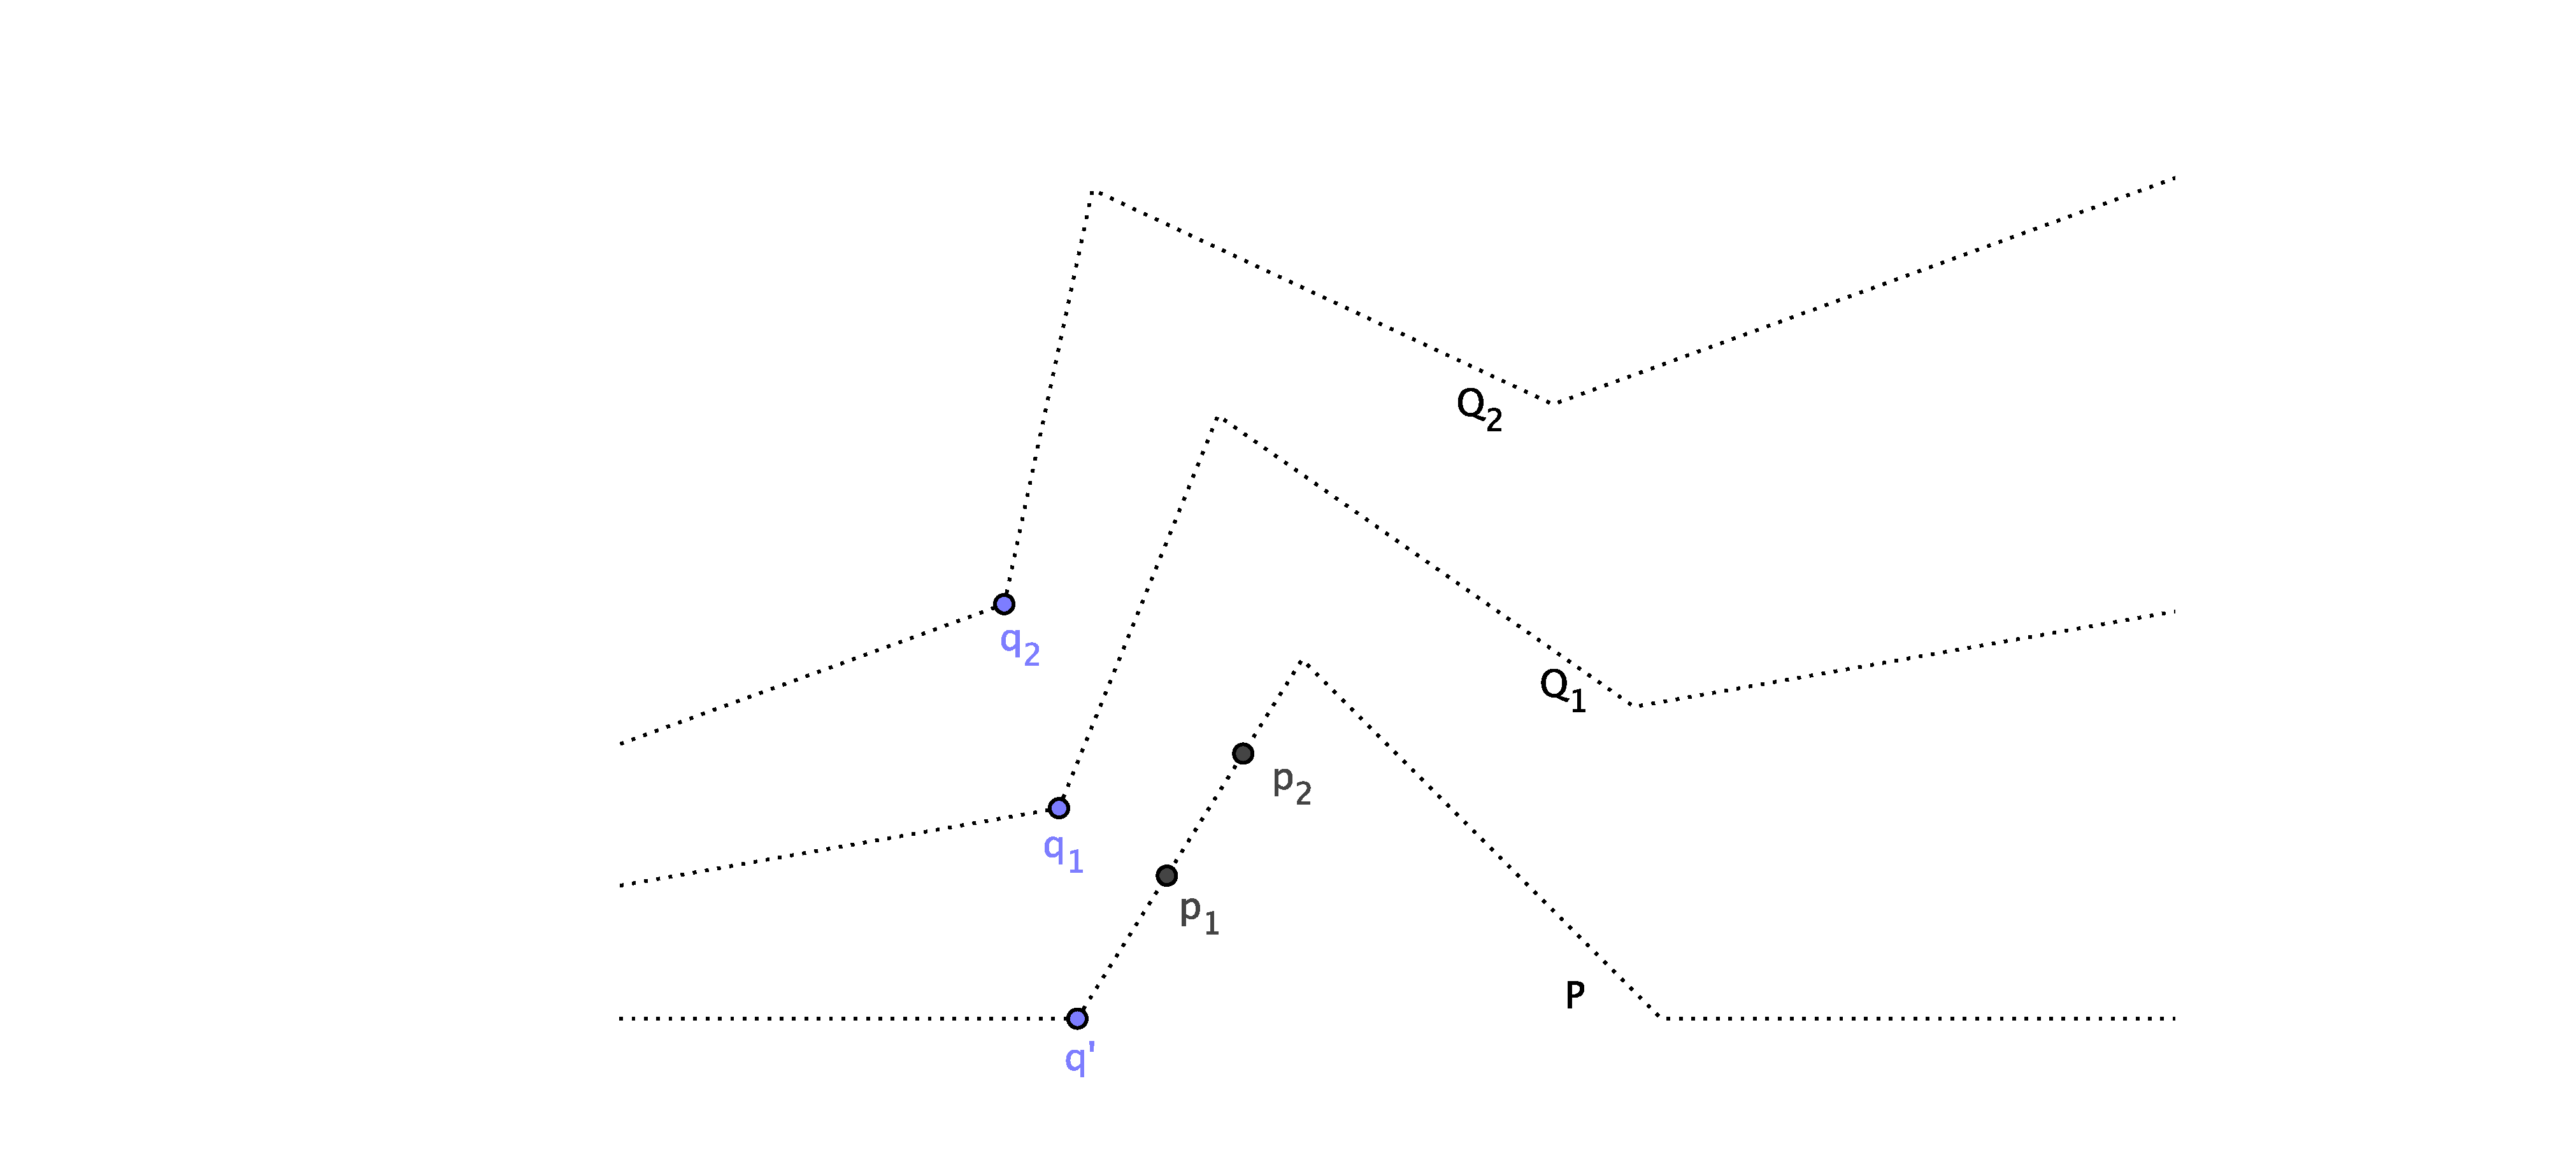
\includegraphics[width=.5\textwidth]{fig/icp_true_approx_cor.pdf}
\caption{Single point at two ICP iterations}
\label{fig:icp_true_approx_cor}
\end{wrapfigure}
The figure shows a fixed point cloud $P$, and a loose point cloud $Q$ at two different alignments, $Q_1$ being aligned more accurately than $Q_2$. $q_2, q_1, q'$ represent the same position in the coordinate systems of the three point clouds. $q \in Q$, but in general $q' \notin P$ except when $Q$ and $P$ have exactly the same constellation.
$p_1, p_2 \in P$ are the correspondence points chosen for $q_1$ and $q_2$ by the closest point criterion.

Hypothesis (1) translates into $d(q_1, q') < d(q_2, q') \Rightarrow d(p_1, q') < d(p_2, q')$. If the point clouds consisted only of the line $\bar{q' p_1}$ this would be true from the triangle similarity. Clearly $\lim_{q \rightarrow q'} d(p, q) = 0$. But the convergence is generally not monotonous. For example if $q$ were to come in from another angle, $p$ could oscillate between the closest points from the two segments adjacent to $q'$.

The error minimization step pulls all $q_i$ closer to $q_i$. Because $\{ p_i \}$ and $\{ q_i \}$ have different constellations, they cannot be made to coincide, but $d(p_i, q_i)$ will get smaller in the least squares sense. \footnote{If it were to get larger, then $\matr{I}$ would be a better transformation estimation than the one found by least squares minimization.} This shows that $d(q_1, p_2) < d(q_2, p_2)$. $p_1$ is the closest point to $q_1$ by the closest point criterion, meaning that $q_2$ cannot be closer. Hence $d(q_1, p_1) < d(q_1, p_2) < d(q_2, p_2)$. This proves the convergence of the ICP algorithm with the closest point criterion.

For hypothesis (2) to be satisfied, it must additionally be true that $d(q', p_1) < d(q', q_2)$. When this is not true, the algorithm can converge towards a local minimum.



\subsubsection{Local minima}
ICP minimizes an error function $e : \mathbb{R}^6 \rightarrow \mathbb{R}$ taking as input a rigid transformation, which can be represented using $6$ independent variables. The function $e$ is different at each iteration, and depends on the correspondences.


\subsection{Generalized ICP}
Conceptually, the difference between point-to-point ICP and point-to-plane ICP is that in the point-to-plane variant, the position of a point on a surface has no impact on the error metric and minimization. This is useful because the point clouds represent solid surfaces approximated using a discrete set of points, and the goal of a registration algorithm is to align those surfaces, and not the points that represent it. The registration algorithm should be agnostic to the distribution of points on a surface.

\emph{Generalized ICP}, first described in \cite{Sega2009}, is a generalization that covers both these variants. Each point is replaced by a gaussian probability distribution that models the uncertainty of its position on the surface and orthogonal to the surface. From this a new error metric formula to minimize is deduced that includes covariance matrices for the two points' distributions.


\section{Coarse Registration}
For coarse registration, no initial alignment of the point clouds is used, and the goal is to obtain an approximative alignment of matching point clouds, which can then be improved upon using fine registration. 

\subsection{Manual registration}
Most commonly, coarse registration is done manually. One method is to define at least three pairs of corresponding positions in the two point clouds, another to rotate and translate the point clouds using a 3D interface.

Both methods can be time consuming because one works using a two-dimensional projection of the two point clouds on a computer screen, the view is difficult to recognize when they incorrectly overlap, and one needs to be able to rotate and translate both the camera and the two point clouds. For these reasons automatic solutions can be preferred in practice, especially when the scanning project consists of many point clouds.
